\documentclass[a4paper,12pt]{article}
\usepackage[utf8]{inputenc}
\usepackage{amsmath}
\usepackage{graphicx}
\usepackage{hyperref}
\usepackage{tikz}
\usepackage{caption}
\usepackage{xcolor}
\usepackage{listings}
\usepackage{float}
\usepackage{geometry}
\usepackage{times}
\usepackage{titlesec}
\usepackage{booktabs}
\usepackage{multirow}
\usepackage{array}
\usetikzlibrary{positioning, arrows.meta}

% Configuración de página
\geometry{margin=2.5cm}
\setlength{\parskip}{1ex plus 0.5ex minus 0.5ex}

% Colores corporativos
\definecolor{primary}{RGB}{41,128,185}
\definecolor{secondary}{RGB}{52,152,219}
\definecolor{accent}{RGB}{231,76,60}
\definecolor{background}{RGB}{245,245,245}

% Estilos de sección
\titleformat{\section}
{\color{primary}\normalfont\large\bfseries}{\thesection}{1em}{}

% Título
\title{\textbf{Informe de Agenda Distribuido: Arquitectura RAFT con Sharding y WebSockets}}

\date{\today}

\begin{document}

\maketitle

\begin{abstract}
Este informe describe el diseño, organización, y ejecución de un sistema distribuido basado en la arquitectura RAFT con sharding especializado, que incluye la replicación de datos, manejo de eventos en tiempo real, y el uso de WebSockets para notificaciones. Se detallan las principales funcionalidades del sistema, los procesos involucrados, y las decisiones tomadas para garantizar la consistencia, disponibilidad, y seguridad del sistema. El informe también aborda aspectos relacionados con la tolerancia a fallos completa y la replicación de datos en un entorno distribuido mediante el protocolo RAFT combinado con particionamiento inteligente.
\end{abstract}

\tableofcontents
\newpage

\section{Arquitectura del Sistema}
El sistema distribuido se basa en una arquitectura \textbf{RAFT} que permite la replicación de datos entre varios nodos. La arquitectura se organiza en varios \textit{shards}, cada uno con un líder y seguidores, siguiendo el principio de consenso de RAFT. El objetivo principal de la arquitectura es garantizar la consistencia de los datos en presencia de fallos, mediante la replicación de los logs de eventos.

El sistema también incluye un \textit{layer} de notificaciones en tiempo real basado en el patrón \textbf{Pub/Sub} utilizando WebSockets. Cada usuario está suscrito a un canal de eventos de su interés, lo que permite una comunicación eficiente entre los usuarios del sistema.

\subsection{Principios Fundamentales de la Arquitectura}

\subsubsection{RAFT para Datos de Agenda}
\begin{itemize}
    \item \textbf{Elección de líder} para consistencia fuerte en eventos
    \item \textbf{Replicación de logs} para no perder datos
    \item \textbf{Failover automático} cuando un nodo falla
\end{itemize}

\subsubsection{PUB/SUB para Notificaciones}
\begin{itemize}
    \item \textbf{WebSockets} para notificaciones en tiempo real
    \item \textbf{Usuarios suscritos} a sus canales de interés
    \item \textbf{Desacoplado} del almacenamiento de datos
\end{itemize}

\subsubsection{Tolerancia a Fallos Completa}
El sistema está diseñado para proporcionar tolerancia a fallos completa mediante la combinación de múltiples patrones y tecnologías.

\begin{figure}[htbp]
\centering
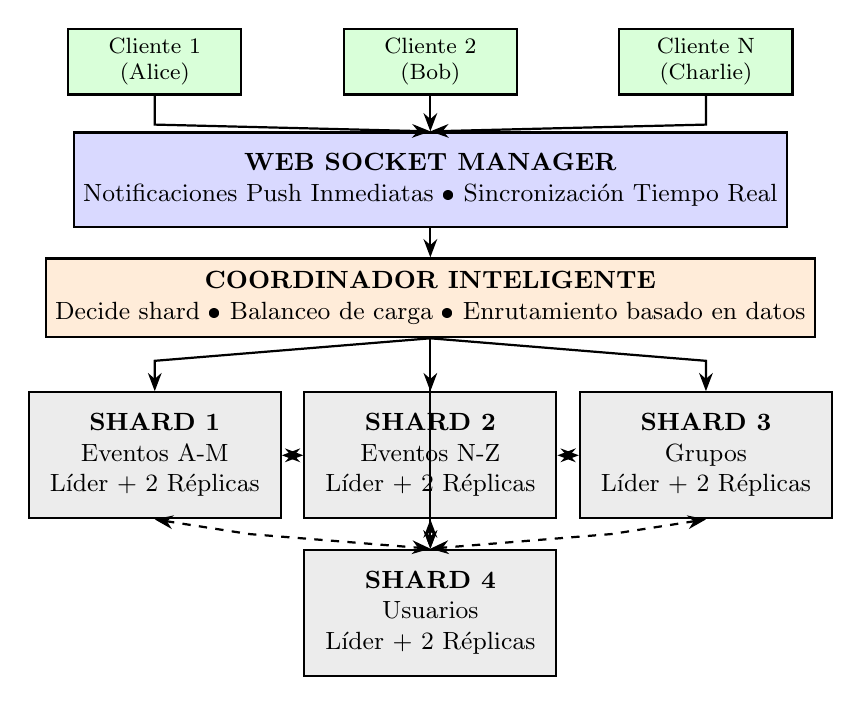
\begin{tikzpicture}[
    raftgroup/.style={rectangle, draw=black, thick, fill=gray!15, minimum width=3.2cm, minimum height=1.6cm, align=center, font=\small},
    pubsub/.style={rectangle, draw=black, thick, fill=blue!15, minimum width=8cm, minimum height=1.2cm, align=center, font=\small},
    client/.style={rectangle, draw=black, thick, fill=green!15, minimum width=2.2cm, minimum height=0.8cm, align=center, font=\footnotesize},
    coordinator/.style={rectangle, draw=black, thick, fill=orange!15, minimum width=8cm, minimum height=1cm, align=center, font=\small},
    arrow/.style={-Stealth, thick},
    doublearrow/.style={<->, thick, >=Stealth}
]

% Clientes
\node[client] (client1) at (0,0) {Cliente 1 \\ (Alice)};
\node[client] (client2) at (3.5,0) {Cliente 2 \\ (Bob)};
\node[client] (client3) at (7,0) {Cliente N \\ (Charlie)};

% WebSocket Manager
\node[pubsub] (websocket) at (3.5,-1.5) {\textbf{WEB SOCKET MANAGER} \\ Notificaciones Push Inmediatas • Sincronización Tiempo Real};

% Coordinador Inteligente
\node[coordinator] (coordinator) at (3.5,-3) {\textbf{COORDINADOR INTELIGENTE} \\ Decide shard • Balanceo de carga • Enrutamiento basado en datos};

% Conexiones superiores
\draw[arrow] (client1.south) -- (0,-0.8) -- (websocket.north);
\draw[arrow] (client2.south) -- (websocket.north);
\draw[arrow] (client3.south) -- (7,-0.8) -- (websocket.north);

\draw[arrow] (websocket.south) -- (coordinator.north);

% Grupos RAFT inferiores
\node[raftgroup] (group1) at (0,-5) {\textbf{SHARD 1} \\ Eventos A-M \\ Líder + 2 Réplicas};
\node[raftgroup] (group2) at (3.5,-5) {\textbf{SHARD 2} \\ Eventos N-Z \\ Líder + 2 Réplicas};
\node[raftgroup] (group3) at (7,-5) {\textbf{SHARD 3} \\ Grupos \\ Líder + 2 Réplicas};
\node[raftgroup] (group4) at (3.5,-7) {\textbf{SHARD 4} \\ Usuarios \\ Líder + 2 Réplicas};

% Conexiones del coordinador a shards
\draw[arrow] (coordinator.south) -- (0,-3.8) -- (group1.north);
\draw[arrow] (coordinator.south) -- (group2.north);
\draw[arrow] (coordinator.south) -- (7,-3.8) -- (group3.north);
\draw[arrow] (coordinator.south) -- (3.5,-3.8) -- (group4.north);

% Conexiones entre shards
\draw[doublearrow, dashed] (group1.east) -- (group2.west);
\draw[doublearrow, dashed] (group2.east) -- (group3.west);
\draw[doublearrow, dashed] (group1.south) -- (1.2,-6) -- (group4.north);
\draw[doublearrow, dashed] (group2.south) -- (group4.north);
\draw[doublearrow, dashed] (group3.south) -- (5.8,-6) -- (group4.north);

\end{tikzpicture}
\caption{Arquitectura Completa del Sistema: Clientes → WebSockets → Coordinador → Shards Especializados}
\label{fig:arquitectura}
\end{figure}

\section{Organización del Sistema Distribuido}
El sistema distribuido se organiza en varios componentes clave:

\begin{itemize}
    \item \textbf{Cliente (Streamlit Frontend):} Interfaz de usuario con vistas de login, calendario, eventos, grupos e invitaciones
    \item \textbf{WebSocket Manager:} Administra las conexiones en tiempo real y las notificaciones push inmediatas
    \item \textbf{Coordinador Inteligente:} Decide a qué \textit{shard} va cada operación y balancea la carga entre los \textit{shards}
    \item \textbf{Shards Especializados:} Cada shard gestiona un subconjunto de los datos, como eventos, usuarios, y grupos. Cada shard sigue el protocolo RAFT con un líder y múltiples réplicas
    \item \textbf{Nodos RAFT:} Proporcionan tolerancia a fallos con almacenamiento local, réplica automática y elección de líder
\end{itemize}

\subsection{Detalle de los Shards Especializados}
\begin{table}[htbp]
\centering
\small
\begin{tabular}{p{2.6cm} p{2.2cm} p{2.8cm} p{2.2cm}}
\toprule
\textbf{Shard} & \textbf{Tipo Datos} & \textbf{Particionamiento} & \textbf{Nodos} \\
\midrule
Shard 1 & Eventos & A-M & 3 (Líder + 2 Réplicas) \\
Shard 2 & Eventos & N-Z & 3 (Líder + 2 Réplicas) \\
Shard 3 & Grupos & Todos & 3 (Líder + 2 Réplicas) \\
Shard 4 & Usuarios & Todos & 3 (Líder + 2 Réplicas) \\
\bottomrule
\end{tabular}
\caption{Distribución de shards especializados en el sistema}
\label{tab:shards}
\end{table}

\subsection{Combinación de Patrones y Tecnologías}

\subsubsection{Patrones Implementados}
\begin{itemize}
    \item \textbf{SHARDING (Particionado):} Data Partitioning + Horizontal Scaling
    \item \textbf{RAFT CONSENSUS:} Consensus Algorithm + State Machine Replication  
    \item \textbf{SPECIALIZED LEADERSHIP:} CQRS + Service Specialization
    \item \textbf{PUB/SUB + WEB SOCKETS:} Publish-Subscribe + Real-Time Communication
    \item \textbf{INTELLIGENT ROUTING:} Router + Load Balancer
\end{itemize}

\subsubsection{Esquema de Tecnología}
\begin{center}
\textbf{SHARDING (Escalabilidad) + RAFT (Consistencia)} $\rightarrow$ \\
\textbf{MULTI-LEADER (Rendimiento) + SPECIALIZATION (Eficiencia)} $\rightarrow$ \\
\textbf{REAL-TIME LAYER (Experiencia) + INTELLIGENT ROUTING (Balanceo)}
\end{center}

\section{Flujo Completo de una Operación}

\subsection{Ejemplo: Alice crea un evento}

\begin{figure}[htbp]
\centering
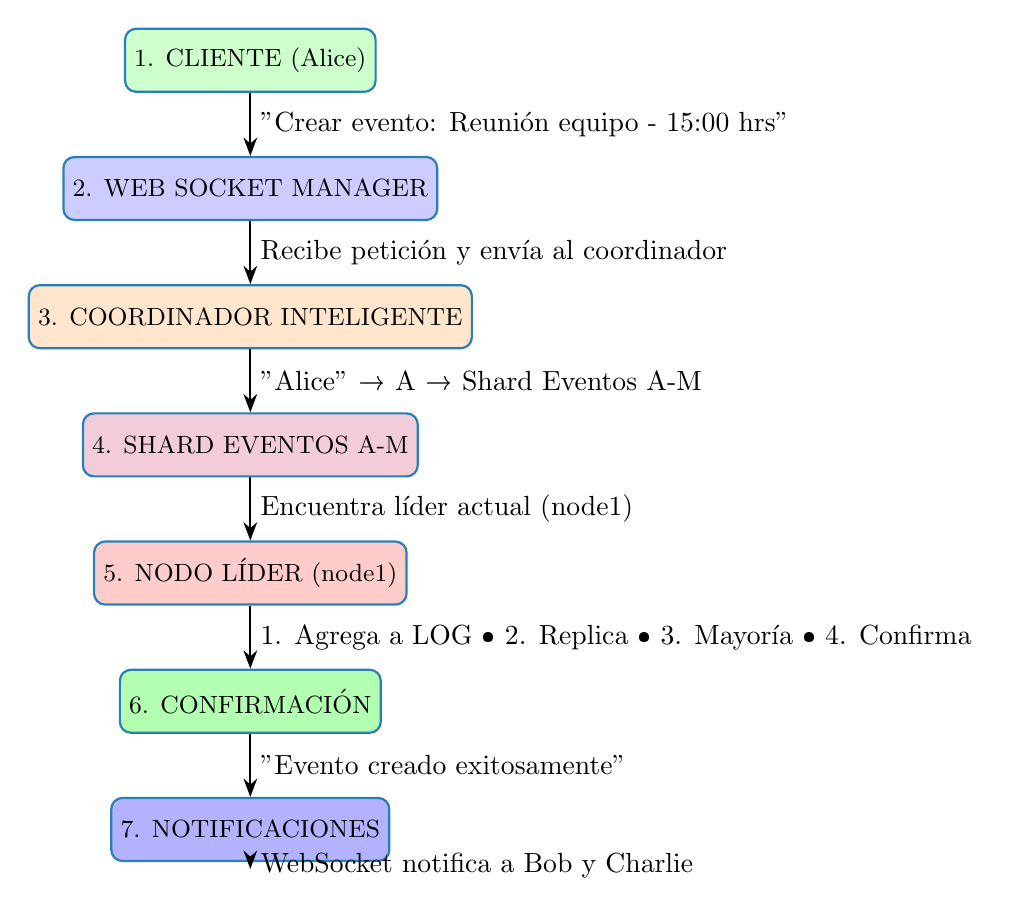
\begin{tikzpicture}[
    stepbox/.style={rectangle, draw=primary, thick, rounded corners, minimum width=3cm, minimum height=0.8cm, align=center, font=\small},
    arrow/.style={-Stealth, thick}
]

\node[stepbox, fill=green!20] (step1) {1. CLIENTE (Alice)};
\node[stepbox, fill=blue!20, below=0.8cm of step1] (step2) {2. WEB SOCKET MANAGER};
\node[stepbox, fill=orange!20, below=0.8cm of step2] (step3) {3. COORDINADOR INTELIGENTE};
\node[stepbox, fill=purple!20, below=0.8cm of step3] (step4) {4. SHARD EVENTOS A-M};
\node[stepbox, fill=red!20, below=0.8cm of step4] (step5) {5. NODO LÍDER (node1)};
\node[stepbox, fill=green!30, below=0.8cm of step5] (step6) {6. CONFIRMACIÓN};
\node[stepbox, fill=blue!30, below=0.8cm of step6] (step7) {7. NOTIFICACIONES};

\draw[arrow] (step1) -- node[right] {"Crear evento: Reunión equipo - 15:00 hrs"} (step2);
\draw[arrow] (step2) -- node[right] {Recibe petición y envía al coordinador} (step3);
\draw[arrow] (step3) -- node[right] {"Alice" → A → Shard Eventos A-M} (step4);
\draw[arrow] (step4) -- node[right] {Encuentra líder actual (node1)} (step5);
\draw[arrow] (step5) -- node[right] {1. Agrega a LOG • 2. Replica • 3. Mayoría • 4. Confirma} (step6);
\draw[arrow] (step6) -- node[right] {"Evento creado exitosamente"} (step7);
\draw[arrow] (step7) -- node[right] {WebSocket notifica a Bob y Charlie} +(0,-0.5);

\end{tikzpicture}
\caption{Flujo detallado de creación de evento por Alice}
\label{fig:flujo}
\end{figure}

\subsection{Proceso Detallado en el Nodo Líder}
Cuando el nodo líder recibe una operación:
\begin{enumerate}
    \item \textbf{Agrega operación} a su LOG local
    \item \textbf{Replica} a los 2 nodos seguidores (node4, node7)
    \item \textbf{Espera confirmación} de mayoría (2/3 nodos)
    \item \textbf{Aplica operación} y confirma al cliente
\end{enumerate}

\section{Tolerancia a Fallos y Recuperación}

\subsection{Mecanismo de Failover Automático}
\subsubsection{Escenario: Fallo del Líder del Shard Eventos A-M}

\subsubsection{Escenario: Fallo del Líder del Shard Eventos A-M}

\begin{figure}[htbp]
\centering
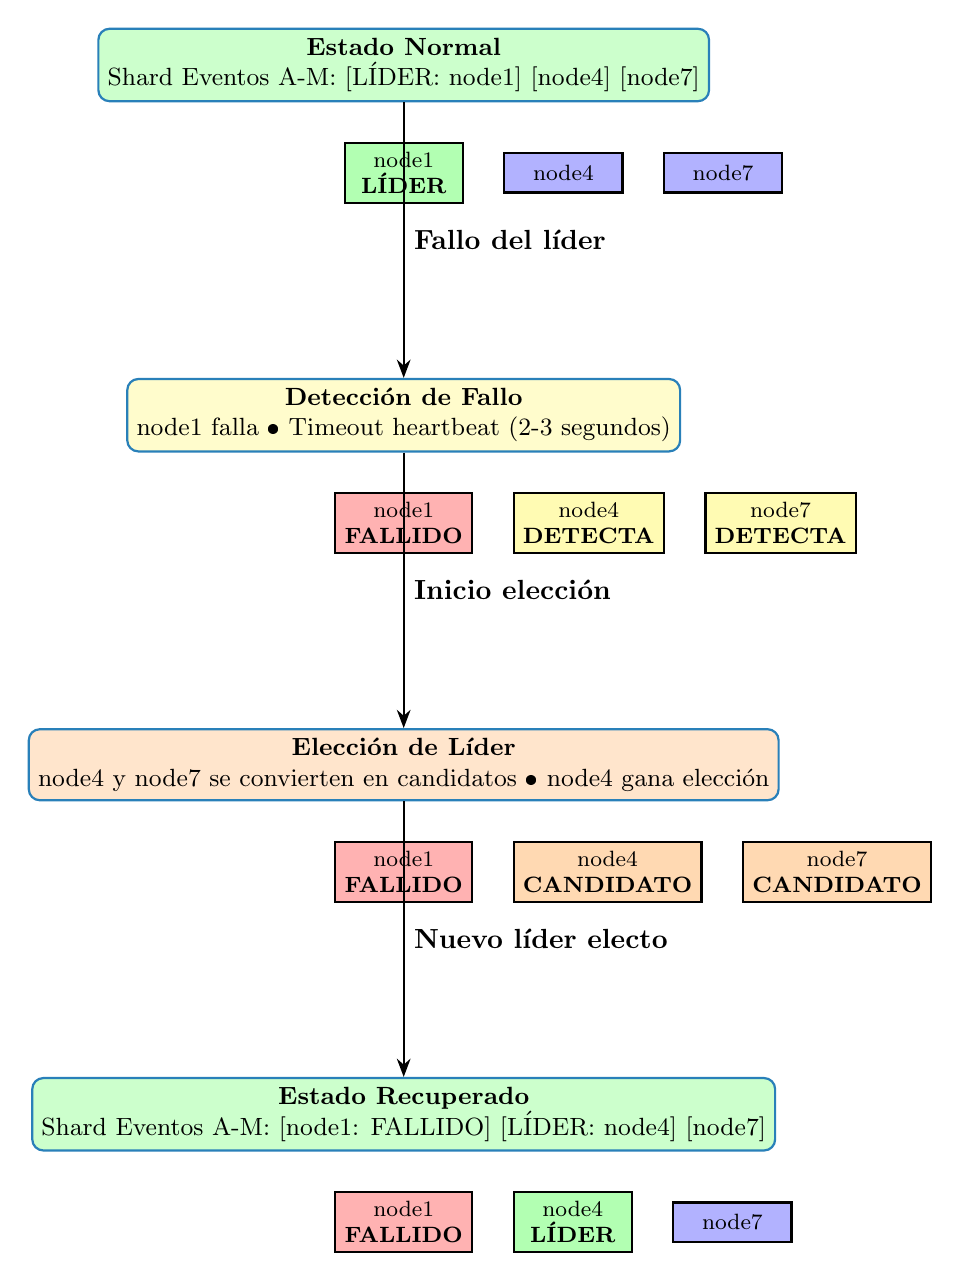
\begin{tikzpicture}[
    state/.style={rectangle, draw=primary, thick, rounded corners, minimum width=6cm, minimum height=0.9cm, align=center, font=\small},
    nodebox/.style={rectangle, draw=black, thick, minimum width=1.5cm, minimum height=0.5cm, align=center, font=\footnotesize},
    arrow/.style={-Stealth, thick}
]

% ========== ESTADO 1: NORMAL ==========
\node[state, fill=green!20] (normal) {\textbf{Estado Normal} \\ Shard Eventos A-M: [LÍDER: node1] [node4] [node7]};

% Nodos en estado normal - más espacio debajo
\node[nodebox, fill=green!30, below=0.5cm of normal] (n1) {node1 \\ \textbf{LÍDER}};
\node[nodebox, fill=blue!30, right=0.5cm of n1] (n4) {node4};
\node[nodebox, fill=blue!30, right=0.5cm of n4] (n7) {node7};

% ========== ESTADO 2: DETECCIÓN ==========
\node[state, fill=yellow!20, below=3.5cm of normal] (detection) {\textbf{Detección de Fallo} \\ node1 falla • Timeout heartbeat (2-3 segundos)};

% Nodos en detección
\node[nodebox, fill=red!30, below=0.5cm of detection] (n1f) {node1 \\ \textbf{FALLIDO}};
\node[nodebox, fill=yellow!30, right=0.5cm of n1f] (n4d) {node4 \\ \textbf{DETECTA}};
\node[nodebox, fill=yellow!30, right=0.5cm of n4d] (n7d) {node7 \\ \textbf{DETECTA}};

% ========== ESTADO 3: ELECCIÓN ==========
\node[state, fill=orange!20, below=3.5cm of detection] (election) {\textbf{Elección de Líder} \\ node4 y node7 se convierten en candidatos • node4 gana elección};

% Nodos en elección
\node[nodebox, fill=red!30, below=0.5cm of election] (n1e) {node1 \\ \textbf{FALLIDO}};
\node[nodebox, fill=orange!30, right=0.5cm of n1e] (n4c) {node4 \\ \textbf{CANDIDATO}};
\node[nodebox, fill=orange!30, right=0.5cm of n4c] (n7c) {node7 \\ \textbf{CANDIDATO}};

% ========== ESTADO 4: RECUPERADO ==========
\node[state, fill=green!20, below=3.5cm of election] (recovered) {\textbf{Estado Recuperado} \\ Shard Eventos A-M: [node1: FALLIDO] [LÍDER: node4] [node7]};

% Nodos en estado recuperado
\node[nodebox, fill=red!30, below=0.5cm of recovered] (n1r) {node1 \\ \textbf{FALLIDO}};
\node[nodebox, fill=green!30, right=0.5cm of n1r] (n4l) {node4 \\ \textbf{LÍDER}};
\node[nodebox, fill=blue!30, right=0.5cm of n4l] (n7r) {node7};

% ========== FLECHAS ==========
\draw[arrow] (normal.south) -- node[right] {\textbf{Fallo del líder}} (detection.north);
\draw[arrow] (detection.south) -- node[right] {\textbf{Inicio elección}} (election.north);
\draw[arrow] (election.south) -- node[right] {\textbf{Nuevo líder electo}} (recovered.north);

\end{tikzpicture}
\caption{Proceso completo de failover automático ante fallo de líder}
\label{fig:failover}
\end{figure}
\subsubsection{Proceso de Recuperación Detallado}
\begin{enumerate}
    \item \textbf{node1 falla} (se desconecta o se apaga)
    \item \textbf{Los seguidores detectan timeout} (no reciben heartbeat por 2-3 segundos)
    \item \textbf{Elección automática:}
    \begin{itemize}
        \item node4 se convierte en CANDIDATO
        \item node7 se convierte en CANDIDATO  
        \item Piden votos entre sí
        \item node4 gana la elección (mayoría)
    \end{itemize}
    \item \textbf{Nuevo líder:} Shard Eventos A-M: [node1: FALLIDO] [LÍDER: node4] [node7]
    \item \textbf{Operaciones continúan:}
    \begin{itemize}
        \item Las nuevas operaciones van a node4
        \item node4 replica a node7
        \item Cuando node1 se recupere, se sincroniza automáticamente
    \end{itemize}
    \item \textbf{Clientes no notan nada:}
    \begin{itemize}
        \item El coordinador redirige automáticamente al nuevo líder
        \item Las operaciones siguen funcionando normalmente
    \end{itemize}
\end{enumerate}

\section{Distribución de Datos y Particionamiento}

\subsection{Cómo se Dividen los Datos}

\begin{table}[H]
\centering
\small
\begin{tabular}{p{2.5cm} p{3cm} p{4.5cm}}
\toprule
\textbf{Usuario/Grupo} & \textbf{Shard Destino} & \textbf{Ejemplo} \\
\midrule
alice & Eventos A-M & Eventos de Alice van al Shard 1 \\
bob & Eventos N-Z & Eventos de Bob van al Shard 2 \\
charlie & Eventos A-M & Eventos de Charlie van al Shard 1 \\
david & Eventos N-Z & Eventos de David van al Shard 2 \\
\midrule
Todos los Grupos & Shard Grupos & Todos los grupos van al Shard 3 \\
Todos los Usuarios & Shard Usuarios & Todos los usuarios van al Shard 4 \\
\bottomrule
\end{tabular}
\caption{Distribución de datos entre shards especializados}
\label{tab:distribucion}
\end{table}

\subsection{Configuración de Nodos y Topología Física}

\subsubsection{Topología con 4 Servidores Físicos}
\begin{table}[H]
\centering
\small
\begin{tabular}{p{2.8cm} p{8.2cm}}
\toprule
\textbf{Servidor} & \textbf{Nodos Alojados} \\
\midrule
Servidor 1 & Shard1-node1, Shard2-node4, Shard3-node7, Shard4-node10 \\
Servidor 2 & Shard1-node4, Shard2-node1, Shard3-node4, Shard4-node7 \\
Servidor 3 & Shard1-node7, Shard2-node7, Shard3-node1, Shard4-node4 \\
Servidor 4 & Shard1-node10, Shard2-node10, Shard3-node10, Shard4-node1 \\
\bottomrule
\end{tabular}
\caption{Distribución de nodos RAFT en servidores físicos para alta disponibilidad}
\label{tab:topologia}
\end{table}

\section{Roles del Sistema}
Cada nodo en el sistema tiene un rol específico dentro del protocolo RAFT. Los roles incluyen:

\begin{itemize}
    \item \textbf{Líder:} El nodo que coordina la replicación de logs y garantiza la consistencia del sistema.
    \item \textbf{Seguidor:} Nodos que siguen al líder y replican sus logs.
    \item \textbf{Candidato:} Nodos que pueden ser elegidos como líderes si el líder actual falla.
\end{itemize}

\section{Distribución de Servicios en Docker}
El sistema distribuido está implementado en contenedores Docker. Cada grupo de RAFT se ejecuta en contenedores separados, con la comunicación entre los nodos facilitada por Docker Swarm.

\subsection{Redes Docker}
\begin{itemize}
    \item \textbf{raft-network:} Red interna para comunicación entre nodos RAFT
    \item \textbf{api-network:} Red para comunicación frontend-backend
    \item \textbf{public-network:} Red para acceso externo de clientes
\end{itemize}

\section{Procesos del Sistema}
El sistema consta de varios procesos que trabajan en conjunto para garantizar el funcionamiento adecuado:

\begin{itemize}
    \item \textbf{Proceso de Elección de Líder:} Los nodos RAFT eligen un líder para garantizar la consistencia de los datos.
    \item \textbf{Replicación de Logs:} El líder replica sus logs a los nodos seguidores.
    \item \textbf{Notificación en Tiempo Real:} Los clientes se suscriben a canales de eventos y reciben notificaciones a través de WebSockets.
\end{itemize}

\section{Comunicación en el Sistema}
El sistema utiliza varios tipos de comunicación:

\begin{itemize}
    \item \textbf{RPC (Remote Procedure Call):} Usado en el protocolo RAFT para la replicación de logs y la elección de líder.
    \item \textbf{WebSockets:} Usados para la comunicación en tiempo real entre el servidor y los clientes.
    \item \textbf{REST API:} Usada para interactuar con la base de datos del sistema y para la creación y gestión de eventos.
\end{itemize}

\subsection{Flujo de Comunicación}
\begin{enumerate}
    \item Cliente envía solicitud vía WebSocket/REST
    \item Coordinador enruta al shard correspondiente
    \item Líder del shard procesa y replica la operación
    \item Confirmación enviada al cliente
    \item Notificaciones broadcast a clientes interesados
\end{enumerate}

\section{Coordinación del Sistema}
El sistema garantiza que todos los servicios estén sincronizados:

\begin{itemize}
    \item \textbf{Sincronización de Acciones:} A través de RAFT, el líder asegura que las operaciones se apliquen en todos los nodos.
    \item \textbf{Acceso Exclusivo a Recursos:} Se asegura que solo un nodo líder pueda modificar los datos, evitando condiciones de carrera.
\end{itemize}

\section{Seguridad}
La seguridad del sistema se aborda en dos niveles:

\begin{itemize}
    \item \textbf{Seguridad en la Comunicación:} Las comunicaciones entre nodos y clientes están protegidas mediante WebSockets seguros (wss://).
    \item \textbf{Autenticación y Autorización:} Los usuarios deben autenticar su sesión para interactuar con el sistema, y los accesos están restringidos según los roles (líder, miembro, etc.).
\end{itemize}

\subsection{Medidas de Seguridad Implementadas}
\begin{itemize}
    \item Autenticación JWT para usuarios
    \item Encriptación TLS/SSL en todas las comunicaciones
    \item Validación de entrada en todos los endpoints
    \item Logs de auditoría para operaciones críticas
\end{itemize}


\end{document}